\documentclass[11pt]{article}

\usepackage{geometry}
\geometry{letterpaper, margin=1in}
\usepackage{graphicx}
\usepackage{booktabs}
\usepackage{amsmath}
\usepackage{microtype}
\usepackage{xcolor}
\usepackage{caption}
\usepackage{float}
\usepackage{enumitem}
\usepackage{array}
\usepackage[hidelinks]{hyperref}

\captionsetup{font=small, labelfont=bf}
\newcommand{\code}[1]{\texttt{#1}}
\setlength{\tabcolsep}{4pt}
\renewcommand{\arraystretch}{1.12}

\title{\vspace{-2.2em}\bfseries Recursive self-improvement for long-running agents\\[0.3em]
\large The problem it solves, how it differs from giving an agent a memory, and what the measurements show so far}

\author{SenseLab Research\\[0.3em]\normalsize\url{https://sense-lab.ai}}
\date{Preprint v0.1, October 2026}

\begin{document}
\sloppy
\maketitle

\begin{abstract}
\noindent
An agent that runs for months acts on knowledge that goes stale, and nobody tells it. A model,
a prompt full of its own history, or a vector store can tell the agent what it did before. None
can tell it that this has stopped working, write the corrected rule, prove it on the failing
cases, release it to a share of traffic and take it back if it does harm. That loop is what we
mean by recursive self-improvement. SenseLab's engine implements it in four levels, and this
paper reports what it measured on a preregistered benchmark in which the correct action for a
task class changes part way through, for half of the class only. On four held-out seeds, two
agent models and two task families (1,600 episodes per system), the engine takes the new
action first in 45\,\% of the episodes whose rule moved, against 25\,\% for the model alone,
32--36\,\% for three pgvector variants and 40\,\% for a 24k-token context window; it wins 8 to
11 of 16 paired cells against each, no pairing survives Holm correction, and the gain is
concentrated in \code{support}. It holds the classes that did not change at 100\,\% against
77\,\% for the model alone, at a third of the cost of the context window; on the kept half,
the rule that did not move within a changed class, the context window is ahead of the engine
(92\,\% against 69\,\%). On development seeds, a joining agent was right on 122
of 122 first exposures (strongest retrieval baseline 68--75\,\%), and in an exploratory run the
gate shipped four corrections and stopped a wrong one at 88\,\% recurrence against 10\,\%.
Inside a 100-episode cell the gates add nothing measurable to the engine's first level, outcome
attribution; that level is more than a win/loss count, since the engine beats a DIY outcome
counter by 13 points on the moved half and 16 on the unchanged classes. The four levels are one
loop; where we know which level carried a number, we say so.
\end{abstract}

\section{The problem}
\label{sec:problem}

Most evaluations of agents measure one task at a time. A model reads a task, acts, and is
scored. Deployment is different in one way that matters more than any other: the agent keeps
going. A support agent handles tickets for a year. A CI agent repairs builds for every commit a
team pushes. An operations agent runs the same procedure every night. Over that time the world
the agent works in changes, and almost none of the changes arrive as instructions.

Three properties of this setting decide what kind of system can work in it.

\begin{itemize}[leftmargin=1.4em, itemsep=2pt]
\item \emph{Tasks do not repeat.} Every ticket, build failure and incident is a new instance.
Nothing can be memorised verbatim; what carries over is the rule, ``in this situation, take
this action''.
\item \emph{Rules change silently and partially.} A policy is rewritten for one tier of
customer and kept for the rest. A dependency is pinned for one class of package and left alone
for others. The agent's old rule is now right half of the time, which is the hardest case: a
system that only demotes what failed has no signal, because the rule still succeeds often enough
to look fine.
\item \emph{The cost of a wrong rule compounds.} An agent that acts on a stale rule fails on
every later instance of that situation, and so does every other agent that reads the same
rule. A fleet of ten agents sharing one record repeats one mistake ten times per round.
\end{itemize}

The failure that matters is a confident action on what used to be true, repeated until a
person notices. The question for anyone building agents for
long-running work is how the system itself can notice, correct and verify, without a person in
every loop, and without making things worse when its correction is wrong.

\section{Three ways to keep an agent current, and where each stops}
\label{sec:alternatives}

The approaches in use today put the burden in three different places.

\paragraph{Trust the model.} The agent runs on a frontier model with a fixed prompt. Everything
it knows about the operation is what the model learned in pretraining plus what the prompt
says. This is the baseline every deployment starts from. It has one strength: the model's
default policy is usually the textbook one, and when the operation follows the textbook the agent
is right. It has one weakness that the benchmark below makes concrete: when the operation's rule
differs from the textbook, the model has no way to learn that. In our confirmatory run, the
frontier model alone takes the correct post-change action first in 25\,\% of the episodes whose
rule moved and in 27\,\% of the episodes in the changed classes whose rule did not move.
In the \code{support} family its moved-half rate is 0 of 150. It never learns the house rule
because it has nowhere to write it.

\paragraph{Put the record in the prompt.} The agent is given its own history: every prior note
and outcome from the operation, most recent first, as many as fit. The model then reasons over
the record. This works well on one thing. When a rule is non-standard and has not changed, the
record is full of consistent examples and the model follows them: 92\,\% on the kept half in our
run, the best of any system by a wide margin. It fails on the thing this paper is about. When a
rule has changed, the record contradicts itself, old successes against new failures, and the
model has to work out from raw history which half is current. It does so in 40\,\% of moved-half
episodes. The approach also has two structural limits. The record grows without bound and must
be truncated (24k tokens here), so the oldest evidence is the first to go, and every episode
pays to re-read everything: \$0.130 per episode, three times the cost of the engine and nine
times the cost of the model alone. And it does not transfer: what one agent has in its prompt is
invisible to the next agent until it is copied there.

\paragraph{Retrieve from a vector store.} The agent writes notes after each task, embeds them,
and retrieves the nearest ones before the next task. This is what most ``agent memory'' systems
are~\cite{reflexion,expel,awm}, with variations: a cross-encoder reranker to sharpen retrieval, or a per-entry win/loss
counter so the agent can see how often a note led to success. We ran all three. Plain pgvector
retrieval takes the new action first in 32\,\% of moved-half episodes; with a reranker, 36\,\%;
with the win/loss counter, 32\,\%. All three keep an unchanged non-standard rule at 58--66\,\%,
well below the context window's 92\,\%. The reason is in what retrieval answers. A vector store
answers ``what did I write that looks like this?''. It does not answer ``is what I wrote still
true?''. A reranker makes the first answer sharper and leaves the second unasked. A win/loss
counter is a step toward the second answer, and in our run it did not help on the moved half and
cost 12 points on the unchanged classes (84\,\% against 96\,\% for plain retrieval). A counter on
an entry says how often it worked. It does not say when, or what to do instead. Hosted memory
products were not run here; an earlier grid on the same benchmark family ran
Mem0~\cite{senselab-cl}.

The common thread is that all three treat knowledge as something to store and recall. What they
leave out is a process: something that watches whether recalled knowledge still works, writes
the corrected rule when it does not, tests the correction, and releases it carefully. That
process is the subject of the next section.

\section{What recursive self-improvement means here}
\label{sec:rsi}

We use the term in a narrow, operational sense. A system is recursively self-improving when its
own outcomes change the knowledge it acts on, the changes are themselves tested against outcomes
before they take effect, and the machinery that makes the changes is subject to the same
evidence as the knowledge it changes. The word ``recursive'' points at the last clause: the
corrections apply to the thing that produces corrections, and the record the loop keeps is also
what trains its next version.

The term is also used for systems that rewrite their own code or training toward open-ended
capability gain~\cite{godel,dgm}. Nothing here does that. The engine changes the operating
knowledge its agents act on, and the prompts and models that produce corrections to it; every
change is tested against outcomes it did not write, exposed to a share of live traffic before
all of it, reversible, and logged. The gate is the design.

SenseLab's engine implements this as four levels. Everything below is production code; the
benchmark calls the public API and the engine's own scheduler does the rest.

\paragraph{Level 0: outcomes decide what the agent acts on.} Before acting, an agent asks the
engine for a briefing and a retrieval on its situation. As it works it records the actions it
takes and any attempt that failed. When the task ends it commits the outcome. The sealed trace
carries exactly what was read, and the outcome is attributed to it: an entry read by a run that
then failed is charged; an entry read by a clean success is credited. Every entry carries an
evidence status (untested, validated, contested, discredited), and retrieval returns, with each
hit, how each candidate action has fared here on similar tasks and a recommendation: act,
explore, or escalate. The ``explore'' recommendation is assigned per agent, so ten agents facing
the same uncertainty try different things instead of the same one.

This level already differs from a vector store in kind. The store answers by similarity. Level~0
answers by evidence attached to the similar thing, and that evidence comes from outcomes the
engine observed, including the agent's own failed attempts. A rule that was validated three
times and then fails is flagged as a \emph{regime shift}: the world moved under a rule that used
to be right. The engine also scopes the shift to a \emph{situation}, a canonical label the agent
attaches to each session, so a rule that broke for the paid tier is not demoted for the free
tier.

\paragraph{Level 1: the engine proposes, tests and ships corrections.} A regime shift proposes a
fix automatically. SenseLab's repair agent, a platform-side component of the engine, reads the
failing runs, the entry and the loop's history on that entry, and drafts either a corrected
entry or a conditional procedure (conditions, steps, a verify step) on a branch of the shared
record. It attaches a manifest: the runs it predicts it repairs, the runs it must not break, and
an expected prevention rate. Nothing on the branch is visible to agents yet.

The draft then has to pass three gates.
\begin{enumerate}[leftmargin=1.6em, itemsep=2pt]
\item \emph{Stand-in replay.} A stand-in model re-runs each manifest case with the branch as its
memory and the tool calls answered from the recorded run. A replay that could not be answered
from the record (fidelity below 0.5) does not count as a pass.
\item \emph{The customer's own replay.} The case set is delivered to the customer's agent, which
re-runs it on the branch. The fix must turn the failed runs into successes and must not break the
passed ones. A success reached only after a recorded failed attempt fails the case.
\item \emph{A live canary.} Sessions are bucketed by a hash of (fix, session); a share reads from
the branch, the rest from the main record, and writes always go to main. The canary is the harm
gate~\cite{kohavi}: the replays prove the benefit on the runs that failed, and the canary has to
show that the change does not make the agent worse on the live traffic the old rule still
served. It passes
when the canary arm recurs significantly less than control, or when a one-sided 95\,\% bound on
the difference in recurrence is under a 10-point margin while the failure is still live in
control. It fails when the canary arm recurs significantly more.
\end{enumerate}
A fix that passes is merged into the main record. Its prevention is verified over the following
window and a fix that regresses is rolled back to the pre-fix versions. A policy can instead
ship on a passed replay, skipping the canary; that is the ``$-$~canary'' ablation below. A set
of continuous judges grades sealed traffic and opens incidents, the second source of proposals
after regime shifts.

\paragraph{Level 2: the loop reads its own history.} Every event in a fix's life (proposed,
tested, replayed, shipped, regressed, rolled back) is written back as evidence on the entry it
concerned, and the repair agent's next draft on that entry reads it. A loop that proposes the
same wrong fix twice has not learned; this level is where it can.

\paragraph{Level 3: the record trains the next model and the next improver.} The traces the
loop produces, including the repair trajectories and the cases they pinned, are a training set.
Smaller models are distilled from them and served with the same evidence record as their memory.
The repair prompt itself is A/B tested across proposals and scored by proven fixes.

\paragraph{Why the gate is the point.} A model that drafts fixes from failure evidence will draft
wrong ones. In the exploratory run reported below, one draft said that a timed-out export should
be split into date ranges; the rule had moved to a settings change, and the draft would have
failed 88\,\% of the sessions it touched. A system that writes such a draft directly into what
every agent reads damages every session at once. The discipline that makes self-improvement
usable in production is the order of operations: evidence before proposal, proof before release,
a small exposure before full exposure, reversibility after, and an audit trail throughout.
Generating corrections is the easy part; the model does that. The engine's value is in refusing
most of them, and in keeping a record of what it refused and why.

\section{What the measurements show}
\label{sec:evidence}

The numbers in this section come from a preregistered study of the whole engine
\cite{rsi-paper}. The hypotheses, arms, metrics, seeds and analysis were registered before the
first run; two seeds were used for development and four held-out seeds ran once after the
analysis code was frozen. This paper quotes the confirmatory read, and labels the two
development-seed probes and the one exploratory run as such.

The analysis was frozen; the engine was not. Defects in the loop's evidence path that the study
found were fixed in production between runs, and every run carries the engine cut it ran on.
Table~\ref{tab:headline} is the fleet-1 confirmatory read: sixteen cells per system, run
01:42--08:19Z on 2026-09-30. One engine cut fell inside that window (\code{post-canary-zero},
03:40Z), with 4,867 of the 12,791 episodes before it. No SenseLab cell straddles the cut: the
\code{support} cells on GPT-5.5 ran on the earlier cut, and every \code{ci-fix} cell and every
Claude Opus~5 cell ran on the later one. Because no cell ran on both, the two engine versions
cannot be compared on the same cells; what can be said is which cells ran on which. On the
earlier-cut cells alone the moved-half difference between SenseLab and every other system is
$+28/{+}11/{+}6/{+}18/{+}23$ points, against $+19/{+}4/{+}13/{+}9/{+}13$ on the full read; the
two differ in composition, since the earlier-cut cells are the \code{support}/GPT-5.5 slice,
where the model alone is at 0\,\% and the context window at 17\,\%, and the full read adds
\code{ci-fix}, where the context window leads. The ten-agent cells of Figure~\ref{fig:curve} and the
exploratory run both ran on the later \code{post-replay-evidence} cut, after the last defect
was fixed. The cut of every run is listed in the companion paper's reproducibility
section~\cite{rsi-paper}.

\paragraph{The benchmark.} Two task families with tool-using agents and oracle-graded outcomes:
\code{support} (a helpdesk agent with account, order and export tools; 15 issue classes) and
\code{ci-fix} (an agent repairing failing CI on a repository; 10 failure classes). Every task
instance is generated and never repeated, with random identifiers so nothing can be read off an
id. Each cell is one agent identity working 100 episodes with one store seeded with 300
distractor entries. At episode 30 the correct action for a subset of classes changes
\emph{conditionally}: it moves for instances with one attribute value (the \emph{moved half})
and stays for the others (the \emph{kept half}). Half of the post-change tasks come from the
changed classes. Classes that did not change are the third population (\emph{unchanged}). The
design was chosen because on an unconditional change outcome learning alone recovers nearly
everything; the conditional change is the case where demotion has no signal, because the old
rule is still right half of the time.

Six systems ran on identical prompts and the same two agent models (GPT-5.5 and Claude Opus~5):
the frontier model alone; the context window (every prior note and outcome, most recent first,
24k tokens); pgvector (bge-small embeddings, cosine top-5 over notes); pgvector with the
cross-encoder reranker SenseLab serves; pgvector with notes, periodic LLM consolidation and a
per-entry win/loss counter shown to the agent (the ``DIY outcomes'' arm); and SenseLab, the
whole engine with corrections shipped only after a passed canary. Four seeds, two families and
two models give sixteen cells per system, 1,600 episodes each. The primary endpoint is
first-attempt success on the moved half after the change; the secondary endpoints are
first-attempt success on the kept half and on the unchanged classes.

\subsection{After the rule changes}

\begin{table}[t]
\centering\footnotesize
\caption{Confirmatory read, sixteen cells per system (4 seeds $\times$ 2 families $\times$ 2
models), 1,600 episodes per system. First-attempt success before the change and, after it, on
the three populations; episode success counts an episode solved within the retry budget of
three; escalated is the share of episodes the agent handed off; cost is the all-in dollar cost
per episode, including for SenseLab the loop's judges, replays and drafts.}
\label{tab:headline}
\setlength{\tabcolsep}{2.6pt}
\begin{tabular}{@{}lrrrrrrr@{}}
\toprule
system & pre-change & moved half & kept half & unchanged & episode & escalated & \$/ep.\\
\midrule
Frontier alone            & 65\,\% & 25\,\% (72/284)  & 27\,\% (75/276)  & 77\,\% (432/560)  & 85.1\,\% & 14.9\,\% & 0.014\\
Context window (24k)      & 86\,\% & 40\,\% (115/284) & 92\,\% (253/276) & 97\,\% (542/560)  & 92.2\,\% &  7.7\,\% & 0.130\\
pgvector                  & 82\,\% & 32\,\% (91/284)  & 66\,\% (183/276) & 96\,\% (539/560)  & 91.8\,\% &  8.2\,\% & 0.024\\
pgvector + rerank         & 77\,\% & 36\,\% (101/284) & 66\,\% (183/276) & 91\,\% (511/560)  & 89.7\,\% & 10.3\,\% & 0.027\\
pgvector + outcomes (DIY) & 76\,\% & 32\,\% (90/284)  & 58\,\% (161/276) & 84\,\% (470/560)  & 88.2\,\% & 11.8\,\% & 0.032\\
SenseLab                  & 85\,\% & 45\,\% (127/283) & 69\,\% (191/276) & 100\,\% (556/557) & 95.2\,\% &  5.0\,\% & 0.042\\
\bottomrule
\end{tabular}
\end{table}

\begin{figure}[t]
\centering
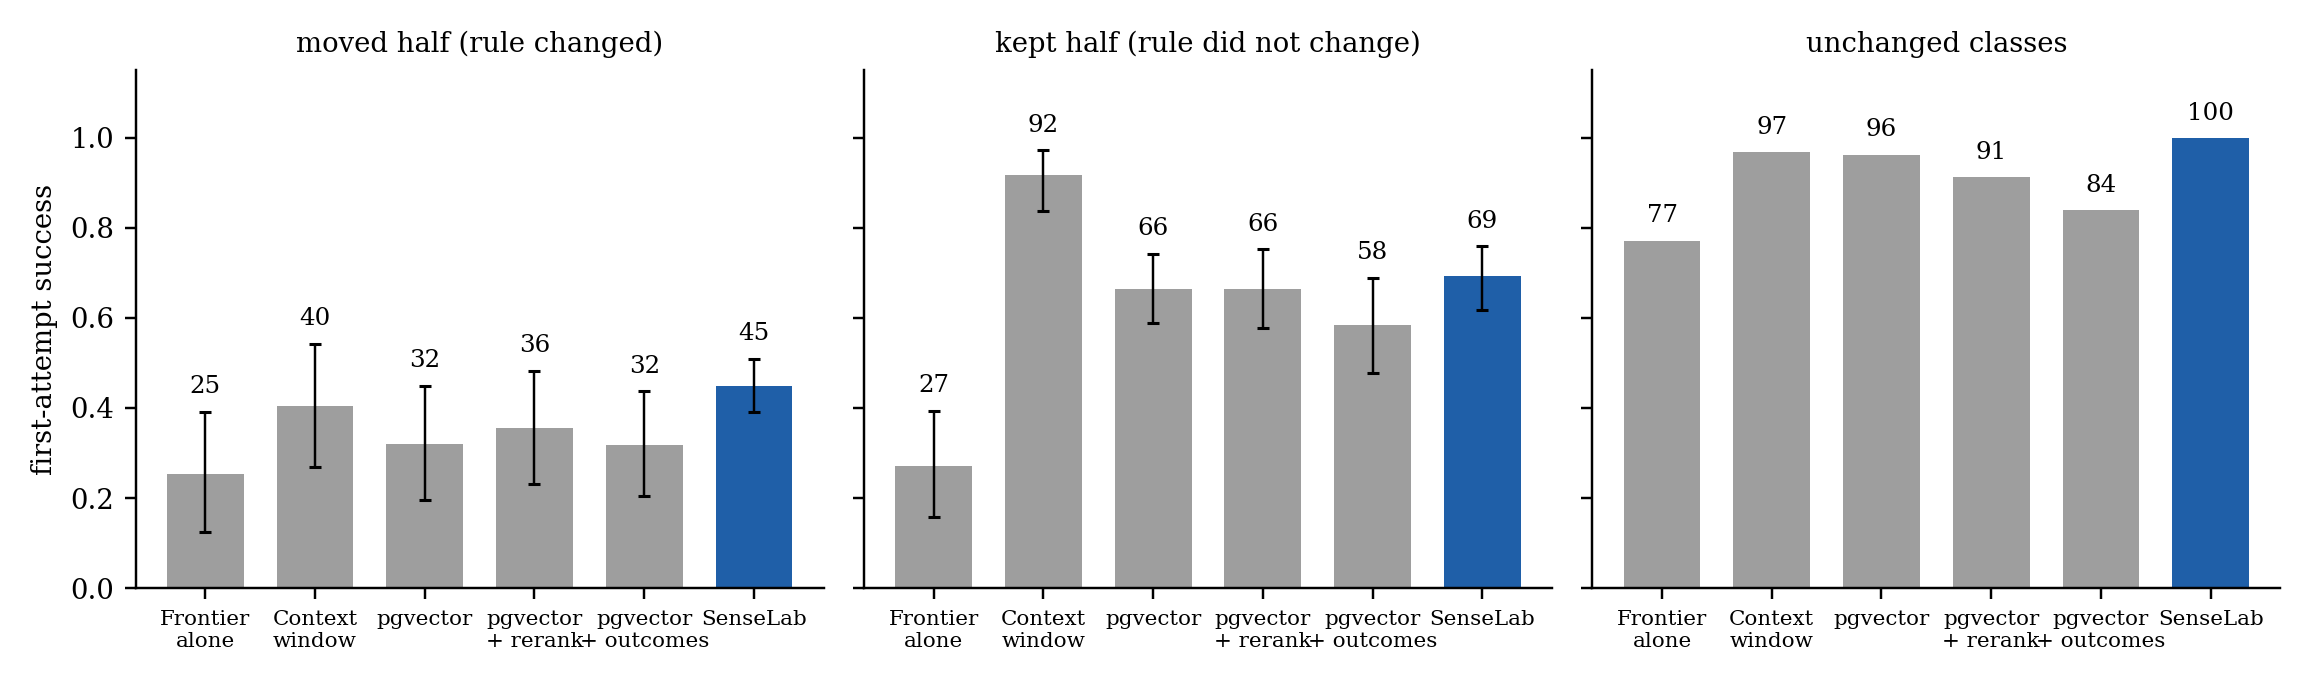
\includegraphics[width=\textwidth]{figures/pos_headline.png}
\caption{The three populations of Table~\ref{tab:headline}. Bars are first-attempt success
after the change; whiskers on the moved and kept halves are cell-level bootstrap intervals over
the sixteen cells.}
\label{fig:headline}
\end{figure}

Table~\ref{tab:headline} and Figure~\ref{fig:headline} carry the main result. Before the change
every system with a store is at 76--86\,\% and the model alone at 65\,\%: a store of any kind
teaches the house rules. After the change the systems separate on the population the change
created. On the moved half SenseLab takes the new action first in 45\,\% of episodes
(127/283, cell-level interval [39, 51]); the context window is at 40\,\%, the pgvector arms at
32--36\,\%, the model alone at 25\,\%. On the unchanged classes SenseLab is at 100\,\% (556/557)
and no system is above it. On the kept half the context window is ahead (92\,\% against
69\,\%), and the engine is level with the pgvector arms.

Paired on (family, seed, model) over the sixteen cells, SenseLab's moved-half rate is above
every other system: $+19$ points over the model alone, $+4$ over the context window, $+13$ over
pgvector, $+9$ over pgvector with the reranker and $+13$ over the DIY outcome store, winning 8
to 11 of the 16 cells in each pairing. The exact sign-flip test gives $p = 0.024$ against the
model alone, $0.040$ against pgvector and the DIY store, $0.119$ against the reranker and
$0.544$ against the context window; after Holm correction across the five comparisons none is
below 0.05 (0.121, 0.544, 0.159, 0.239, 0.159). The sign is right in every pairing and the
sizes match the development seeds; sixteen cells is the power this study bought. The reader
should take the deltas as estimates with their intervals, and the context-window comparison on
the moved half as undecided.

The secondary endpoints are cleaner. On the unchanged classes SenseLab is above the model alone
($+23$, Holm $0.002$), the reranker ($+9$, $0.035$) and the DIY store ($+16$, $0.004$), and
indistinguishable from the context window and plain pgvector. On the kept half it is above the
model alone by 38 points (14 of 16 cells, Holm $0.007$), level with the three pgvector arms, and
24 points below the context window (1 of 16 cells, Holm $0.001$). That last number is a real
cost of the approach and we return to it in \S\ref{sec:limits}.

\paragraph{Where the gap is large.} The moved half is the primary endpoint because it is the
hardest population, and there the engine's lead is modest. On the other endpoints the lead is
not modest, and Table~\ref{tab:gaps} collects the ones a reader deciding what to deploy should
weigh. One miss in 557 on the classes whose rule did not change: 100\,\% against 77\,\% for the
model alone, 84\,\% for the DIY outcome store and 91\,\% for the reranker, all three
separations surviving Holm. Forty-two points over the model alone on the \code{support} moved
half, where every system without an outcome record is at 27\,\% or less and the model alone
never takes the new action. A third fewer escalations than the next-best system and a third as
many as the model alone: 80 hand-offs in 1,592 episodes against 124 for the context window and
238 for the model alone. The highest episode success of any system, 95.2\,\%, with a retry budget of three.
Twenty points over the model alone before any rule changes, because the engine's record teaches
the house rules an agent is deployed into. And on Claude Opus~5 the moved-half lead over the
context window is nine points, where on GPT-5.5 the two are level.

\begin{table}[t]
\centering\footnotesize
\caption{Where the confirmatory gaps are large. Rates over the sixteen cells; Holm-corrected
$p$ from the preregistered paired sign-flip test where the comparison is one of the registered
secondary endpoints, blank otherwise.}
\label{tab:gaps}
\setlength{\tabcolsep}{4pt}
\begin{tabular}{@{}lrrrr@{}}
\toprule
endpoint & SenseLab & against & gap & Holm $p$\\
\midrule
unchanged classes, first attempt    & 100\,\% (556/557) & Frontier alone 77\,\%          & $+23$ pts & 0.002\\
                                    &                     & pgvector + outcomes 84\,\%     & $+16$ pts & 0.004\\
                                    &                     & pgvector + rerank 91\,\%       & $+9$ pts  & 0.035\\
kept half, first attempt            & 69\,\% (191/276)  & Frontier alone 27\,\%          & $+38$ pts & 0.007\\
\code{support} moved half           & 42\,\% (62/149)   & Frontier alone 0\,\% (0/150)   & $+42$ pts & \\
                                    &                     & best other (rerank) 27\,\%     & $+15$ pts & \\
moved half, Claude Opus~5           & 54\,\% (76/141)   & Context window 45\,\%          & $+9$ pts  & \\
pre-change first attempt            & 85\,\% (406/480)  & Frontier alone 65\,\%          & $+20$ pts & \\
episode success (retry budget 3)    & 95.2\,\%          & Context window 92.2\,\%        & $+3$ pts  & \\
                                    &                     & Frontier alone 85.1\,\%        & $+10$ pts & \\
escalations                         & 5.0\,\% (80)      & Context window 7.7\,\% (124)   & $-35\,\%$ & \\
                                    &                     & Frontier alone 14.9\,\% (238)  & $-66\,\%$ & \\
cost per episode, all in            & \$0.042            & Context window \$0.130          & $3.1\times$ cheaper & \\
\bottomrule
\end{tabular}
\end{table}

\paragraph{Where the gain comes from.} The moved-half result is a \code{support} result. There
SenseLab is at 42\,\% (62/149) against 0--27\,\% for every other system, with the model alone at
0 of 150: on house rules that differ from the textbook and then move, nothing without an
outcome record learns the new rule at all. On \code{ci-fix} SenseLab is at 49\,\% (65/134)
against 43--67\,\%, behind the context window (67\,\%). The two families differ in what the
textbook gets right: in \code{ci-fix} the frontier model alone is at 54\,\% on the moved half,
which suggests the post-change action is close to its default, and at 5\,\% (7/146) on the kept
half, where a house rule it never learned still applies. By model, SenseLab is level with
the context window on GPT-5.5 (36\,\% both) and ahead on Claude Opus~5 (54\,\% against 45\,\%);
the pgvector arms swap order between the models (13--27\,\% on GPT-5.5, 37--51\,\% on Opus). The
engine's effect does not depend on which model reads it.

\subsection{The long horizon: ten agents, 200 episodes}

A 100-episode cell with one agent is short for a loop whose gates need graded live traffic. The
second protocol runs ten agents against one shared engine for 200 episodes, with the change at
episode 50, on the same four held-out seeds, both families, GPT-5.5 (eight cells, 1,600
episodes). It is reported descriptively, as registered, and it has no baseline: no pgvector or
context-window fleet ran under this protocol, so the curve compares the engine with its own
earlier episodes, and a shared store of any kind might climb as evidence accumulates. What the
protocol adds that the single-agent cells cannot is the gate's behaviour with ten agents' traffic,
reported next.

\begin{figure}[t]
\centering
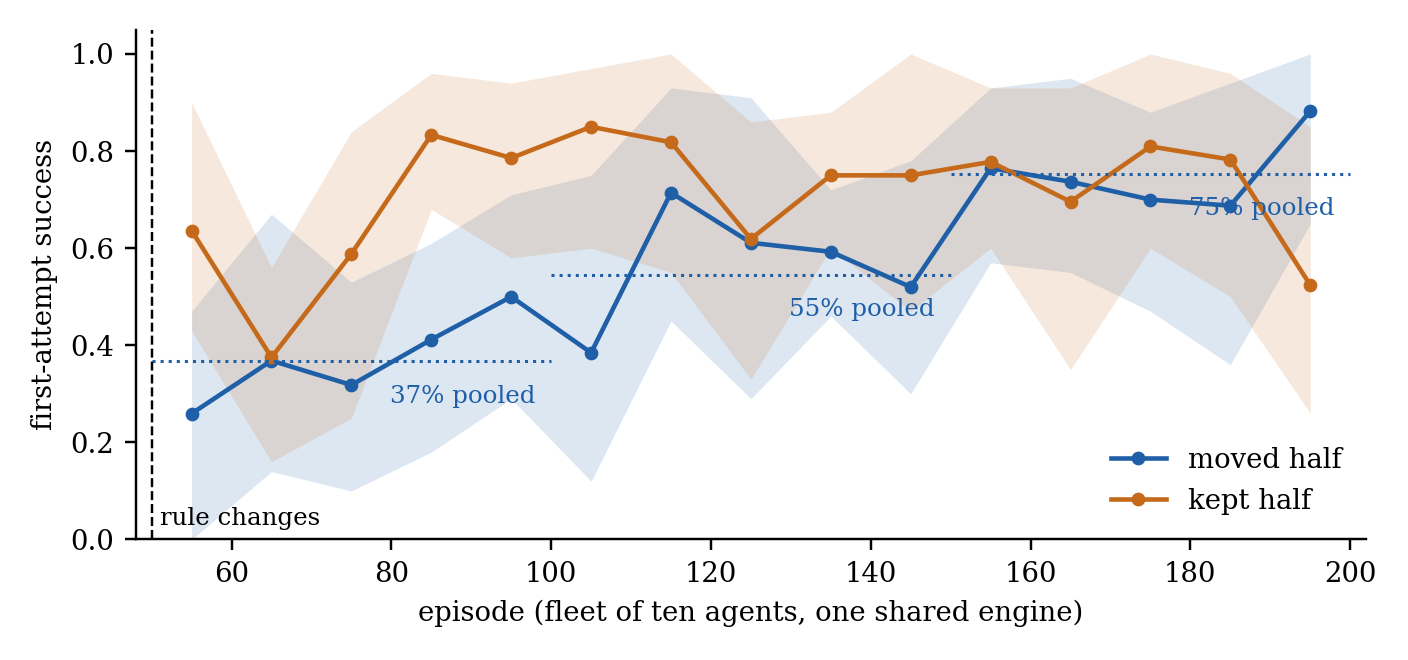
\includegraphics[width=0.78\textwidth]{figures/pos_curve.png}
\caption{Fleet of ten agents sharing one engine, 200 episodes, change at episode 50; eight
confirmatory cells pooled. First-attempt success per ten-episode block on the moved and kept
halves, with cell-level bootstrap bands; dotted lines are the pooled moved-half rate over each
fifty-episode window. No baseline system ran under this protocol; the curve is descriptive.}
\label{fig:curve}
\end{figure}

Figure~\ref{fig:curve} shows the curve. Pooled over the eight cells, moved-half first-attempt
success is 37\,\% (40/109) in episodes 50--99, 55\,\% (60/110) in 100--149 and 75\,\% (67/89) in
150--199, with 88\,\% (15/17) in the last block. The kept half is 66, 76 and 72\,\% over the same
windows. The unchanged classes are at 100\,\% in every post-change block (594/595). A rule that
moved for half of a class at episode 50 is taken correctly three quarters of the time by episode
150, by ten agents each of which handled about a tenth of the episodes. What each inherits
from the others is the outcome record and whatever the loop wrote.

\subsection{What the loop did, and what it refused}

The engine's own record is the second half of the evidence, and it is where the gate shows.

In the sixteen single-agent cells the loop proposed 32 corrections (23 from a regime shift, 9
from the judges). Sixteen passed the stand-in replay, six passed the customer's replay, five
opened a canary, two shipped and none was reverted. The same loop with the canary removed, so
that a passed replay ships, shipped 10 of 44. The canary held back four fixes in five that the
replay would have released, in cells where no canary could reach a graded decision before the
cell ended. In the eight ten-agent cells the loop proposed 48, the customer's replay passed 6
and failed 38, six canaries opened in six different cells, and none shipped: four reached the
graded floor on both arms, one failed on a zero-count bound at 10 of 10 graded sessions, and
three closed with both arms above the floor and no decision, because at 14 to 20 graded runs per
arm the non-inferiority test cannot close a 10-point margin. The canary arm read its fix in 57 of
76 graded sessions (75\,\%) and the control arm in 0 of 54, so the gate was grading a treated
arm against an untreated one, as designed.

The exploratory run sized the traffic to the gate. On the two development seeds, four cells of
400 episodes with every post-change episode drawn from the changed classes, the loop proposed 68
corrections; the stand-in replay passed 20, the customer's replay passed 8 and failed 22; eight
canaries opened and five decided inside their cells. Four passed and shipped, three of them on a
\code{ci-fix} class the fleet already handled (first-attempt success 0.89--0.97 before the
ships, 0.89--0.96 after), so what the gate certified there is that the correction did no harm.
One failed. The draft ``csv export timeout $\to$ split date ranges'' was the wrong action under
the changed rule, which had moved to a settings change. Its canary arm graded 8 sessions, read
the fix in 7, and recurred in 7 (88\,\%) against 2 of 20 in control (10\,\%; $p < 0.001$). The
loop wrote the failure as a lesson to the main record within a second, the branch never reached
main, and the next draft the repair agent produced for that class named the settings action.
Nobody injected this case. It came out of the loop's own proposals, and the gate caught it.

\paragraph{What did not separate.} Inside a 100-episode cell with one agent, the engine without
its canary and the engine without its repair loop are indistinguishable from the whole engine:
44 / 71 / 99\,\% and 43 / 68 / 99\,\% (moved / kept / unchanged) against 45 / 69 / 100. Level~0,
the outcome record, does most of the measurable work at this horizon. The repair loop's
contribution is visible in its lifecycle counts and in the exploratory canary, and in the shape
of the ten-agent curve; it is not visible in the single-agent aggregate. We say so because the
case for the loop has to rest on what it prevents as much as on what it adds, and the former is
only measurable where it has traffic.

Level~0 is not a win/loss counter. The DIY outcome arm is the naive version of it: notes,
periodic consolidation, and a per-entry success count shown to the agent. The engine beats
that arm by 13 points on the moved half (10 of 16 cells, $p = 0.040$ before correction), by 16
on the unchanged classes (Holm $0.004$) and by 8 on the kept half, and escalates less than half
as often (5.0\,\% against 11.8\,\%); the ablation with the repair loop switched off, which is
level~0 by itself, is at 43 / 68 / 99\,\% against the DIY arm's 32 / 58 / 84. The difference is
what happens between an outcome and the next retrieval. The engine attributes each outcome to the exact entries the
session read and the attempts it recorded, so a failure charges the rule that was followed and
not every note that happened to be retrieved. It keeps an evidence status per entry, with a
threshold for discrediting and a regime-shift rule (validated at least three times, now
failing) that distinguishes a rule the world moved from a rule that never worked. It scopes all
of that to a situation, so a rule broken for one tier is not demoted for another. And it returns
a recommendation with the hits, act, explore or escalate, with exploration assigned per agent
so a fleet does not repeat one agent's mistake. That machinery is the loop's first level, and
the levels above it exist for the case it cannot see: a rule still right half of the time, which
demotion cannot separate from a rule that works. Which level carried each number is stated
wherever we can tell.

\subsection{When the team grows}
\label{sec:team}

No operation runs one agent for long. A second instance is added for load. Another team points
its own agent at the same tools and the same customers. A new use case is built over the same
systems, by people who were not there when the first agent learned the house rules. Every one of
these agents arrives with the same question on its first day: of everything written down about
this operation, what still holds? With a vector store the answer is whatever the retriever
returns, and the new agent has no way to tell a note that was right last quarter from one that is
right now. With the engine the answer is attached to each entry, because the entries carry the
outcomes of every agent that acted on them.

A development-seed probe measured what a joining agent inherits. Six agents share one record on
the \code{support} and \code{ci-fix} families, two seeds, with an unconditional rule change at
episode 20. In the \emph{pioneer} protocol one agent works alone for 60 episodes and five join;
in the \emph{newcomer} protocol five work from the start and a sixth joins at 60. The joiner is
a new identity; it has none of the veterans' sessions. Table~\ref{tab:join} is the read.

\begin{table}[t]
\centering\footnotesize
\caption{A joining agent's first exposure to each task class after it joins (development seeds,
set~A, six agents; pgvector + rerank is the strongest retrieval baseline). \emph{Poisoned}: a
failed first attempt with an untested peer note in context and nothing validated. \emph{Parity}:
the joiner's success reaches the veterans' late rate. Tokens are per task the joiner solved.}
\label{tab:join}
\setlength{\tabcolsep}{3pt}
\begin{tabular}{@{}llrrrrrrr@{}}
\toprule
protocol & system & \multicolumn{2}{c}{first exposure} & poisoned & escal. & parity & ep.\ to & tokens /\\
 & & changed & all & & & reached & parity & solved\\
\midrule
pioneer  & SenseLab          & 36/36 (100\,\%) & 90/90 (100\,\%) & 0/90 (0\,\%)  & 0\,\%  & 20/20 & 5    & 4,331\\
         & pgvector + rerank & 11/36 (31\,\%)  & 61/90 (68\,\%)  & 29/90 (32\,\%) & 20\,\% & 16/20 & 5    & 7,556\\
newcomer & SenseLab          & 10/10 (100\,\%) & 32/32 (100\,\%) & 0/32 (0\,\%)  & 0\,\%  & 4/4   & 5    & 4,230\\
         & pgvector + rerank & 4/10 (40\,\%)   & 24/32 (75\,\%)  & 8/32 (25\,\%)  & 16\,\% & 4/4   & 11.5 & 6,836\\
\bottomrule
\end{tabular}
\end{table}

A joiner on the engine took the post-change action on its first exposure to a changed class in
36 of 36 and 10 of 10 cases, and the correct action on every first exposure of any kind, 122 of
122, with no stale picks and no escalations. Over all of its episodes after joining it was at
100\,\% first-attempt success (136/136 and 160/160). A joiner on pgvector with a reranker was at
31\,\% and 40\,\% on the changed classes, 68\,\% and 75\,\% over all first exposures, and 62\,\%
over all of its episodes, with 17\,\% stale picks in the pioneer protocol and 16--20\,\% of first
exposures escalated. The record each joiner read explains the difference. The engine's joiner had
a validated entry in context on every first exposure and was never poisoned. The retrieval
joiner had no evidence status on anything it read, and on 32\,\% and 25\,\% of its first
exposures it failed with an untested note from a veteran in its context; on the changed classes,
69\,\% and 60\,\%. The same notes were in both stores. What the engine's joiner inherited was the
part the store cannot hold: which notes had worked since they were written. Onboarding cost
follows: the engine's joiners all reached the veterans' late success rate, in a median of five
episodes in both protocols; four of the twenty retrieval joiners in the pioneer protocol never
did, and in the newcomer protocol the median was 11.5 episodes and 55k tokens against 22k. Per
task solved, the engine's joiner spent 43\,\% and 38\,\% fewer tokens.

This is a development probe on an unconditional change with six agents and one hundred
episodes, and we report it as such. Its direction is the one the organisation case needs. The
cost of learning a changed rule is paid once, by whichever agent meets it first, and every agent
that joins afterwards, on the same team or another, starts from the validated record instead of
from the veterans' unverified notes.

\subsection{Models trained on the record}
\label{sec:models}

The record a team's agents produce is also a training set, and this is level~3 of the engine.
SenseLab builds \emph{Managed Models}: smaller models that SenseLab fine-tunes on a team's own
sealed traces, what the agents read, what they did, what came of it, and the repair
trajectories and pinned cases the loop produced along the way. The trained model is then served
with the same evidence record as its memory. Three things follow for the team. It owns the
intelligence: the record was produced by its agents on its operation, and the model trained on
that record belongs to it, on no vendor's roadmap. It can retrain as the record grows, so a
rule the fleet learned this month is in the next model, and a rule the loop corrected is in it
too. And the model it runs on is a fraction of the cost of the frontier model it learned from.

The first rung of this was measured on the development seeds. Two \code{senselab-s1} students
were trained on 200 sealed \code{support} traces each from the development cells, one on the
whole engine's traces and one on traces from the ablation with the repair loop switched off,
and evaluated on three further held-out seeds (1,500 episodes) in three conditions: the student
alone, the student served with the engine's record, and GPT-5.5 served with the same record.
Table~\ref{tab:student} is the read.

\begin{table}[t]
\centering\footnotesize
\caption{Managed Models at the first rung of the evaluation ladder (development seeds 11 and 23
for training; seeds 101, 113 and 127 for evaluation; \code{support}, set~C, 300 episodes per
condition and model). First-attempt success by population, post-change episodes pooled over the
three seeds ($n$ = 54 moved, 51 kept, 105 unchanged, 90 pre-change per row); cost is agent cost
per episode.}
\label{tab:student}
\setlength{\tabcolsep}{4pt}
\begin{tabular}{@{}llrrrrr@{}}
\toprule
model & memory & moved half & kept half & unchanged & pre-change & \$/episode\\
\midrule
student (engine traces)   & none     & 9\,\%  & 88\,\%  & 69\,\% & 80\,\% & 0.0007\\
student (ablation traces) & none     & 0\,\%  & 100\,\% & 90\,\% & 94\,\% & 0.0007\\
student (engine traces)   & SenseLab & 33\,\% & 69\,\%  & 98\,\% & 71\,\% & 0.0015\\
student (ablation traces) & SenseLab & 30\,\% & 65\,\%  & 97\,\% & 84\,\% & 0.0017\\
GPT-5.5                   & SenseLab & 22\,\% & 69\,\%  & 99\,\% & 80\,\% & 0.0348\\
\bottomrule
\end{tabular}
\end{table}

Alone, the students have learned the house rules and nothing usable about the change: 88\,\%
and 100\,\% on the kept half, 9\,\% and 0\,\% on the moved half. (The engine-trained student
alone does reach the right answer on 96\,\% of moved-half episodes, in 2.1 attempts on average:
it has learned its teacher's recovery path, the stale action first and then the one the
environment accepted, and replays it.) A fine-tuned model is a snapshot of the record at
training time, and a snapshot cannot follow a rule that moves after it was taken. Served with
the engine's record, the same students take the new action first in 33\,\% and 30\,\% of
moved-half episodes, 24 and 30 points above themselves alone in every seed, and hold the
unchanged classes at 98\,\% and 97\,\%. Against GPT-5.5 served with the same record they are
8 to 11 points ahead on the moved half, level on the kept half (69 against 69) and on the
unchanged classes (98 against 99), at \$0.0015 against \$0.0348 per episode: 1/23 of the cost. The record
is what moves with the world; the model is what makes acting on it cheap. The record was produced
by one model's outcomes and lifted another, which is the property an organisation needs if it is
to change models without starting over.

Two disclosures belong next to these numbers. This is rung~0 of the ladder: the evaluation seeds
are new but the task classes and wordings are the ones the students trained on, so a student
ahead of the frontier model here is expected and is not yet evidence of generalisation; rungs
1--3, on classes and wordings the students never saw, are registered and not yet run. And both
students were promoted to serving under a relaxed gate; the default promotion gate would have
rejected both on exact agreement with their teacher (0.00 against a floor of 0.45). The difference between the two students, $-7/0/{+}18$ points across the three seeds, is
small and reported as such. What the rung does show is the shape of the offer: a model the team
owns, trained on what its agents learned, that with the record behind it matches a frontier
model on the house rules and the unchanged work and beats it where the rule moved, at a
twenty-third of the cost.

\section{What this means for building agents}
\label{sec:implications}

The measurements support six statements about how to build agents for long-running work.

\paragraph{The unit of improvement is the operating rule.}
What goes stale is a rule of the form ``in this situation, take this action''. Retraining the
model for every policy change is too slow and too coarse; editing the prompt by hand does not
scale past a few agents. The rule is the thing to store, attribute outcomes to, correct, and
test. Everything in Table~\ref{tab:headline} that separates the systems is about how each one
handles that unit.

\paragraph{Evidence attached to knowledge beats more knowledge.} The context window has strictly
more information than the engine: it sees everything. It loses on the moved half because
information without attribution is a contradiction the model has to resolve on every call. The
engine's record is smaller and carries, with each rule, how it has fared since. On the kept half,
where there is no contradiction, more information wins, and this is the engine's clearest
weakness in the data.

\paragraph{The gate matters more than the generator.} The repair agent drafted 68 corrections in
the exploratory run and 32 and 48 in the confirmatory protocols. The customer's replay rejected
most of them. The canary rejected one that the replay had passed and that would have harmed
nine sessions in ten. A system whose corrections are gated by outcomes it did not write itself
can be left running. One that ships on a model's say-so has to be watched.

\paragraph{An organisation learns once.} Agents multiply: more instances on the same team,
other teams on the same tools, new use cases over the same systems. A new agent on the engine
took the correct action on every first exposure measured, 122 of 122, where the strongest
retrieval baseline failed on a quarter to a third of them with a veteran's unverified note in
its context. The curve in Figure~\ref{fig:curve} is ten agents reaching 75\,\% on a rule that
most of them met for the first time after it had already been learned. The cost of learning a
changed rule is paid once per operation, by whichever agent meets it first.

\paragraph{The team owns the intelligence, and can run it on its own model.} The record is
produced by the team's agents on the team's operation, and the Managed Models SenseLab trains
from it are the team's own, retrainable as the record grows. At the first rung measured, a
student served with the record was level with a frontier model on the house rules and the
unchanged work, ahead where the rule moved, and 23 times cheaper. Accuracy comes from the
record, which keeps moving with the world; cost comes from the model, which the team controls.

\paragraph{Self-diagnosis is an output.} The study that produced these numbers found fourteen
things about the engine's own evidence path, twelve of them defects, during the runs: a regime
shift firing on entries that had never been validated, a replay grading on an outcome the agent
reached only after a failed attempt, a canary arm that was not reading the fix it was supposed
to be grading. Each was found because the loop keeps a record that can be checked against ground
truth, each was fixed in production between runs, and each was re-measured on the same
protocol \cite{rsi-paper}. A retrieval benchmark would have seen none of them, because none of
them is about retrieval. A system that improves itself has to be inspectable in exactly this way,
and the record it keeps for its own gates is what makes it so.

\section{Related work}
\label{sec:related}

\paragraph{Agents that improve from experience.} Self-Refine~\cite{selfrefine} and
STaR~\cite{star} improve a model's outputs or its training data within a task or a training run.
Reflexion~\cite{reflexion} writes a verbal reflection after a failed trial for the next trial on
the same task. ExpeL~\cite{expel} distils cross-task insights from past trajectories into text
the agent reads later; Voyager~\cite{voyager} keeps a library of verified skills; Agent Workflow
Memory~\cite{awm} induces reusable workflows from past successes. All of them write something
after an episode that a later episode reads. None attributes later outcomes back to what was
written, none detects that a written rule has stopped holding, and none tests a correction on the
failing cases and on live traffic before every later episode reads it. Those three steps are the
engine.

\paragraph{Self-modifying systems.} Gödel machines~\cite{godel}, the Darwin Gödel
Machine~\cite{dgm} and AlphaEvolve~\cite{alphaevolve} change their own code under a proof or a
benchmark gate. The gate is the shared idea. The object differs: the engine changes operating
knowledge and the prompts and models that produce corrections to it, each change is measured
against a live control arm, and each is reversible.

\paragraph{Release engineering and bandits.} The engine's third gate is a canary release with a
non-inferiority bound, in the tradition of controlled online experiments~\cite{kohavi}. The act, explore and
escalate recommendation that level~0 returns with each retrieval is a bandit over actions within
a situation~\cite{bandits}, with exploration assigned per agent; the engine's contribution is
the attribution that feeds it, not the policy.

\paragraph{Benchmarks.} $\tau$-bench and $\tau^2$-bench~\cite{taubench,tau2bench} evaluate
tool-using agents against fixed rules, and LongMemEval~\cite{longmemeval} evaluates recall over
long histories. Neither changes a rule under the agent and grades what it does next, which is
the measurement this paper rests on.

\section{Limits}
\label{sec:limits}

The evidence has limits, and some of them are findings about the approach.

The moved-half advantage over the context window is 4 points and does not approach
significance ($p = 0.544$ paired). What separates the two systems is cost (3$\times$) and what
each can do for a second agent; this number does not. The kept-half loss to the context window
(24 points, Holm $0.001$) is the price of a selective, outcome-weighted record on a rule that
did not move: the engine revises what the context window replays. Whether that trade is
right depends on how often an operation's rules change, which is an empirical question about the
operation.

Inside a 100-episode single-agent cell, the repair loop and the canary add nothing measurable
to outcome learning. The loop's value is in the ten-agent curve, in what it refused, and in the
one wrong correction it stopped; the single-agent aggregate does not show it, and we do not
claim it does. In the eight confirmatory ten-agent cells nothing shipped at all, because the
canary's rule needs more graded traffic per arm than 200 episodes across ten agents supplied.
The four ships and the one failure come from an exploratory run on development seeds with the
traffic concentrated on the changed classes, and three of the four ships were on a class that
was already at ceiling. The ten-agent curve has no baseline fleet under its protocol, so it
shows that the engine keeps learning over 200 episodes and not that a store without the engine
would not.

The joiner and Managed Model results are development-seed probes: six agents on an
unconditional change for the first, and rung~0 of a four-rung ladder, under a relaxed promotion
gate, for the second. Their confirmatory versions are registered and not yet run.

The benchmark is two families of synthetic tasks with oracle grading and a rule change the
authors wrote. It knows the truth before and after every change, which is what makes the
measurement possible and what makes it an approximation of an operation whose truth nobody
writes down. Horizons are 100 and 200 episodes. The engine's cost per episode is three times the
model alone and 1.3--1.8 times a pgvector store, and a third of the context window.

\section{Conclusion}

An agent that runs for a long time needs more than a place to put what it learned. It needs a
process that notices when what it learned has stopped being true, writes the correction, proves
it on the cases that failed, exposes it to a little live traffic, and keeps or reverts it on the
evidence. That process is recursive self-improvement in the sense this paper uses, and the
measurements here are, to our knowledge, the first of an engine doing it in production code
against baselines that
only store and recall. The engine is ahead on the population the change created, level or ahead
on what did not change, three times cheaper than the strongest baseline, and able to hand what it
learned to a new agent intact, or to a model the team owns at a twenty-third of the cost. It also records what it refused to ship, which
is the part of a self-improving system that lets you trust the rest.

\begin{thebibliography}{99}\small
\bibitem{rsi-paper} SenseLab Research. Recursive self-improvement, gated by evidence: an engine
that lets deployed agents propose, test, canary and ship corrections to their own operating
knowledge, measured where the world changes under them. Preprint v0.3, October 2026. Companion
paper; preregistration \code{HYPOTHESIS\_RSI.md}, analysis tag \code{analysis-freeze-rsi}.
\bibitem{senselab-cl} SenseLab Research. From memory to recursive self-improvement: agents that
learn from outcomes, agents that only remember, and a model trained on what they learned, when
the tasks never repeat and the rules change. Preprint, 2026.
\bibitem{reflexion} N.~Shinn, F.~Cassano, A.~Gopinath, K.~Narasimhan, S.~Yao. Reflexion: Language
agents with verbal reinforcement learning. NeurIPS 2023.
\bibitem{expel} A.~Zhao, D.~Huang, Q.~Xu, M.~Lin, Y.-J.~Liu, G.~Huang. ExpeL: LLM agents are
experiential learners. AAAI 2024 (arXiv:2308.10144).
\bibitem{voyager} G.~Wang et al. Voyager: An open-ended embodied agent with large language models.
TMLR 2024 (arXiv:2305.16291).
\bibitem{awm} Z.~Z.~Wang, J.~Mao, D.~Fried, G.~Neubig. Agent Workflow Memory. arXiv:2409.07429,
2024.
\bibitem{selfrefine} A.~Madaan et al. Self-Refine: Iterative refinement with self-feedback.
NeurIPS 2023.
\bibitem{star} E.~Zelikman, Y.~Wu, J.~Mu, N.~D.~Goodman. STaR: Bootstrapping reasoning with
reasoning. NeurIPS 2022.
\bibitem{godel} J.~Schmidhuber. Gödel machines: Fully self-referential optimal universal
self-improvers. In \emph{Artificial General Intelligence}, Springer, 2007.
\bibitem{dgm} J.~Zhang, S.~Hu, C.~Lu, R.~Lange, J.~Clune. Darwin Gödel Machine: Open-ended
evolution of self-improving agents. arXiv:2505.22954, 2025.
\bibitem{alphaevolve} A.~Novikov et al. AlphaEvolve: A coding agent for scientific and algorithmic
discovery. arXiv:2506.13131, 2025.
\bibitem{kohavi} R.~Kohavi, D.~Tang, Y.~Xu. \emph{Trustworthy Online Controlled Experiments: A
Practical Guide to A/B Testing}. Cambridge University Press, 2020.
\bibitem{bandits} T.~Lattimore, C.~Szepesv\'ari. \emph{Bandit Algorithms}. Cambridge University
Press, 2020.
\bibitem{taubench} S.~Yao, N.~Shinn, P.~Razavi, K.~Narasimhan. $\tau$-bench: A benchmark for
tool-agent-user interaction in real-world domains. arXiv:2406.12045, 2024.
\bibitem{tau2bench} V.~Barres et al. $\tau^2$-bench: Evaluating conversational agents in a
dual-control environment. arXiv:2506.07982, 2025.
\bibitem{longmemeval} D.~Wu et al. LongMemEval: Benchmarking chat assistants on long-term interactive
memory. ICLR 2025.
\end{thebibliography}

\end{document}
